% Phyloage User Guide
%
% For PDF output: pdflatex phyloage.tex
% For HTML output: plastex pyhloage.tex
%
% For Graphics:
% Use PNG format to avoid problems with HTML conversion.
% Recommended size: < 13cm x 18cm (width x height).
% Recommended resolution: 300 dpi.
%
% Use fixed width instead of textwidth, so that plastex can
% recognize the graphics size. For example use
% \includegraphics[width=13cm]{img/haplogroups.png}
% instead of
% \includegraphics[width=\textwidth]{img/haplogroups.png}


\documentclass[12pt,a4paper]{article}
\usepackage[utf8]{inputenc}
\usepackage[russian,english]{babel}
\usepackage[colorlinks=true, urlcolor=blue, linkcolor=blue]{hyperref}
\usepackage{graphicx}

\begin{document}
\begin{titlepage}

\title{Phyloage User Guide}

\author{Dirk Struve\\
phylofriend at projectory.de\\
\href{https://github.com/yogischogi/phyloage/}{https://github.com/yogischogi/phyloage/}}
\date{\today}
\end{titlepage}
\maketitle

\tableofcontents
\section{Introduction}

Phyloage is an experimental program for genetic genealogy
and history research. It combines SNP and Y-STR results to
calculate TMRCA (Time To Most Recent Common Ancestor)
estimates from STR mutational differences.

Since the emergence of next generation sequencing SNP based
phylogenetic trees are rapidly evolving and less attention
is paid to Y-STR mutations. But if we look at the properties
of SNP mutations in detail, we see that they are not without
drawbacks:

\begin{itemize}
\item SNP mutations are extremely stable. Phylogenetic trees
	based on SNPs are highly reliable.
\item Not all SNPs are useful for genealogical purposes
	\cite{YFullMutationRate}. This is problematic for TMRCA
	calculations because wrong SNPs lead to false results.
\item For TMRCA calculations the margins of error are rather large.
	YFull has tried to include only genealgical relevant SNPs
	into their phylogenetic tree \cite{YFullTree} and estimates
	one mutation every 140 years \cite{YFullMutationRate}.
\end{itemize}

It would be nice to have more precise estimates and a second
independent method for TMRCA calculations, that can be used to
verify and complement the results gained by SNP counting.
This could be achieved by using the well known Y-STR mutations.
Their properties are rather different from SNPs:

\begin{itemize}
\item STRs have been used for genetic genealogy for a long
	time. Some specific marker sets are well known and many
	people have tested.
\item Next generation sequencing reveals results for up to
	500 markers. This should give us enhanced precision for
	TMRCA estimates.
\item Time estimates using STRs are often biased towards
	specific lineages that proliferated more than others.
\item STRs mutate back and forth. It is impossible to create
	reliable phylogenetic trees that go back deep into
	history. Furthermore the back and forth mutations lead
	to a saturation effect that invalidates time estimates
	for long time spans (thousands of years).
\end{itemize}

There have been numerous efforts to overcome the disadvantages
of STR counting. A small overview is given in \cite{Ham15}.

Phyloage introduces a new approach. The basic idea is to
start with an SNP based phylogenetic tree, insert the Y-STR
results and calculate modal haplotypes for each node of the
tree. 

In theory this should reduce saturation effects and give
better time estimates for both deep history and genealogical
time frames.

If you use this program, please remember that it is still
highly experimental. At the time I am writing this (March 1,
2016), there is no person on earth who has a long time
experience with 500 Y-STR markers.

\vspace{1em}\noindent
Have fun experimenting!

\vspace{1em} Dirk




\section{Installation}

This guide is mainly targeted towards persons who use Linux Mint
or other Linux versions of the Debian family. Some familiarity
with the use of Linux commands is assumed.

Currently there are no binary distributions available for
Windows or the Mac. Users of these operating systems can
use Phyloage as well, but they will experience some
laborious installation work. The best way is to follow the
instructions provided on the
\href{http://golang.org/}{Go} home page.

The following list applies to Linux users only:

\begin{enumerate}
\item Make sure that the Go programming language is installed.
	If not it can be installed by typing\\
	\texttt{sudo apt-get install golang}
\item Read the Go
	\href{http://golang.org/doc/install}{Getting Started}
	guide. Make sure to set your \emph{GOPATH} variable and
	include it in your \emph{PATH} so that Go programs can be
	found.
\item Fetch the Phyloage program with\\
	\texttt{go get github.com/yogischogi/phyloage}
\item Install the program with\\
	 \texttt{go install github.com/yogischogi/phyloage}
\end{enumerate}


\section{Command Line Options}

Command line options may be given in arbitrary order.

\begin{description}
\item[-help] Prints available program options.

\item[-treein] Filename of the SNP based phylogenetic tree.
\item[-treeout] Filename of the results tree in text format.
\item[-personsin] Filename or directory of files containing the
	persons' Y-STR values. If this is a single file it must contain
	results for multiple persons. The input file format is CSV
    (comma separated values) or text format.

	If a directory is provided for input it must contain multiple
	files in YFull format, each file containing the results for
	a single person. The person's ID is extracted from the filename.

	\emph{personsin} supports multiple file names separated by
	commas.
\item[-mrin] Filename of the mutation rates to use.
\item[-gentime] Generation time.
\item[-cal] Calibration factor.
\end{description}


\section{Examples}

\subsection{Using YFull Results}

\subsubsection*{SNP Input Tree}

Before you can start you need to create a phylogenetic tree,
that contains SNPs and the IDs of the genetic samples. The
file format is text based and looks like this:

\begin{verbatim}
// This is an example tree.
// Comments begin with //.

CTS4528, S1200
    S11481
        id:YF01234
        id:YF00301
        id:YF02016
    S14328
        id:YF04242
        id:YF00101
        id:YF01010
\end{verbatim}

Each line of the tree contains one or more SNPs or a sample
ID. Subclades and samples are indented by using tabs. Each
sample starts with \texttt{id:} followed by the ID. In our case
these are typical YFull IDs but Phyloage supports Family Tree
DNA data as well. Phyloage uses the Phylofriend
\cite{Phylofriend} program for data import and many
calculations as well. See the Phylofriend User Guide
\cite{PhylofriendUserGuide} for the details of the supported
input formats.

To create a results tree:

\begin{enumerate}
\item Save the input tree to a file, for example \emph{tree.txt}.
\item Download the Y-STR results for the samples from YFull
    and put them into a separate directory, for example
    \emph{allsamples}
\item Execute the following command from a command line
    (the file \emph{111-average.txt} can be found in the
    \emph{mutationrates} directory of the Phylofriend program
    \cite{Phylofriend}):\\
\texttt{phyloage -treein tree.txt -treeout results.txt\\
-personsin allsamples -mrin 111-average.txt -gentime 32}
\end{enumerate}

The results will be stored in a file named \emph{results.txt}.
We have used average mutation rates for 111 markers and a
generation time of 32 years.


\subsubsection*{Results Tree}

Now the file \emph{results.txt} contains a tree with TMRCA
estimates that looks like this:

\begin{verbatim}
CTS4528, S1200, STRs Downstream: 145, formed: 4644, TMRCA: 4644
    S11481, STR-Count: 140, STRs Downstream: 51, formed: 6141, TMRCA: 1647
        id:YF01234, STR-Count: 30
        id:YF00301, STR-Count: 73
        id:YF02016, STR-Count: 52
    S14328, STR-Count: 17, STRs Downstream: 81, formed: 3148, TMRCA: 2597
        id:YF04242, STR-Count: 72
        id:YF00101, STR-Count: 91
        id:YF01010, STR-Count: 82
\end{verbatim}

Because we have used mutation rates for 111 markers, that
were calibrated by using generations, the \texttt{STR count}
is given in generations. It says for how long a Clade has
existed before it developed any subclades. The
\texttt{STRs Downstream} is a measure for the TMRCA.

\texttt{formed} denotes the age of the clade in years. It is
calculated by adding \texttt{STR count} to \texttt{STRs Downstream}
and multiplying the result by the generation time (the
\texttt{gentime} parameter) and an additional calibration
factor (1 by default).

\texttt{TMRCA} is the same as \texttt{STRs Downstream}. It is
just multiplied by the generation time and the calibration
factor.


\subsection{Mutation Counting on the 500 Marker Scale}

In the previous example we have used the average mutation rates
for 111 markers. It is a good idea to start with those markers
because they are well known and have been used for years.

YFull on the other hand reports up to 500 STR markers. Most persons
get about 400 values out of their Big Y test. So we like to use
them, but keep in mind that we do not have a long time experience
with the 500 marker scale.

The input tree will be exactly the same as before but this time
we execute the command:

\vspace{1ex}\noindent
\texttt{phyloage -treein tree.txt -treeout results.txt\\
-personsin=allsample -mrin=500-count.txt -cal=39 }
\vspace{1ex}

\noindent The above command will do mutation counting using
all markers available and then upscale the results to 500
markers. The \texttt{500-count.txt} contains the mutation rates
for marker counting. It can be found in the Phylofriend
\cite{Phylofriend} \emph{mutationrates} directory.

Currently it seems like one mutation counts as 39 years
using Phylofriend's mutation model. So a calibration factor
of 39 is used.


\subsection{Adding Family Tree DNA Results}

It is possible to add Family Tree DNA results to the input
tree. This is very useful if some persons only did test on
the 67 or 111 marker scale. It is also possible to add 12 or
37 marker results but the average mutation rates are different
and the margins of error are very high. So I do not recommend
it.

To add Family Tree DNA results, just insert their IDs
(kit numbers) into the input tree. In this example we add
12345 and 67890 to the input tree:

\begin{verbatim}
CTS4528, S1200
    S11481
        id:YF01234
        id:YF00301
        id:YF02016
        id:12345
        id:67890
    S14328
        id:YF04242
        id:YF00101
        id:YF01010
\end{verbatim}

To create the results tree:

\begin{enumerate}
\item Save the input tree to the file \emph{tree.txt}.
\item Put the YFull results into a directory named
	\emph{yfull}.
\item Save the Family Tree DNA results in a spreadsheet
	called \emph{cts4528.csv}. The first column of the 
	spreadsheet must contain the Family Tree DNA kit numbers.
	For additional details about the file format, please
	consult the Phylofriend User Guide \cite{PhylofriendUserGuide}.
\item Execute the following command from a command line:\\
	\texttt{phyloage -treein tree.txt -treeout results.txt\\
	-personsin yfull,cts4528.csv -mrin 111-average.txt\\
	-gentime 32}
\end{enumerate}

The results can be found in the file \emph{results.txt}.
Of course it is also possible to build a tree only from
Family Tree DNA samples and completely leave out YFull
results.


\subsection{Pure Mutation Counting}

If you do not have files containing detailed genetic results,
but you know the number of the individual (private) STR
mutations, it is possible to use the input tree for counting.
Just add the STR numbers to the tree like this (you can also
use this method for SNP counting):

\begin{verbatim}
CTS4528, S1200
    S11481, STR-Count: 2
        id:YF01234, STR-Count: 30
        id:YF00301, STR-Count: 40
        id:YF02016, STR-Count: 50
    S14328, STR-Count: 2
        id:YF04242, STR-Count: 30
        id:YF00101, STR-Count: 40
        id:YF01010, STR-Count: 50
\end{verbatim}


In this example we assume that one mutation counts as 100
years. Thus we use a calibration factor of 100. To create
the result tree, type:

\vspace{1ex}\noindent
\texttt{phyloage -treein tree.txt -treeout results.txt -cal 100}
\vspace{1ex}

\noindent
The result tree contains TMRCA estimates for all clades:

\begin{verbatim}
CTS4528, S1200, STRs Downstream: 42, formed: 4200, TMRCA: 4200
    S11481, STR-Count: 2, STRs Downstream: 40, formed: 4200, TMRCA: 4000
        id:YF01234, STR-Count: 30
        id:YF00301, STR-Count: 40
        id:YF02016, STR-Count: 50
    S14328, STR-Count: 2, STRs Downstream: 40, formed: 4200, TMRCA: 4000
        id:YF04242, STR-Count: 30
        id:YF00101, STR-Count: 40
        id:YF01010, STR-Count: 50
\end{verbatim}







\section{Theory}

\subsection{Modal haplotype}

Phyloage uses Y-STR mutation counting to estimate the TMRCA
(Time to Most Recent Common Ancestor) for a group of persons.
This is not an easy task because STR markers jump back and
forth. If a marker has changed from one value to another and
back again we do not know if a mutation has taken place or
not. So for long time spans STR mutation counting does not
work and we get wrong TMRCA estimates. In many cases this
effect can be calculated and compensated as it has been done
in \cite{Kly09}. However this method has it's limits.

Phyloage uses another approach. It combines SNP based phylogenetic
trees and Y-STR counting. Because of the use of SNPs, the
ancestral positions on the phylogenetic tree are well known.
Phyloage tries to calculate the ancestral haplotype for each
ancestor and uses Y-STR mutation counting between those
haplotypes and the modern samples. The calculated haplotypes
are not necessarily identical to the real ancestral values.
So they are called modal haplotypes.

The calculation of a modal haplotype is not always possible.
Figure \ref{modal} illustrates the situation.

\begin{figure}[ht]
\centering
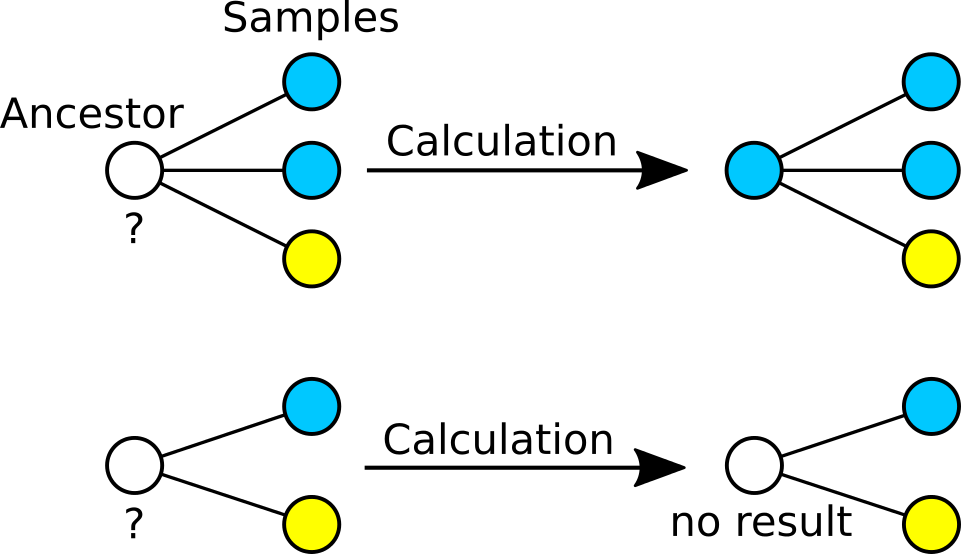
\includegraphics[width=8.14cm]{img/modal.png}
\caption{\label{modal} Calculation of an ancestor's mutational
value from a set of samples. The calculation is only possible
if we have at least three samples.}
\end{figure}

Because mutation rates are usually very slow we may assume
that a mutation occurs rarely. In this case the modal value
of a mutation is identical to the value that occurs most
often among the samples. The rare cases are the mutations.
If the time spans get very long this is no longer true. We
have no idea how many mutations have occurred between the
ancestral haplotype and the modern samples. The mutational
values are just random. If we use them to calculate the modal
haplotype, the result will be different from the real ancestral
values.

So for a valid calculation of a modal haplotype, two
conditions must be satisfied:

\begin{enumerate}
\item We must have at least three samples and two of them must
	have the same mutational value.
\item The time span between two ancestral haplotypes must be
	small compared to the average time in which a mutation occurs.
\end{enumerate}


\subsection{Maximum parsimony method}

As default Phyloage uses an algorithm that tries to satisfy
the maximum parsimony criterion \cite{Wiki-Maximum_parsimony}.
This means that the tree that contains the least amount of
mutations is considered best.

Although this is very intuitive and widely used, it is not
always true or easy to calculate because

\begin{enumerate}
\item In many cases there is no best tree, but a number of
	viable solutions. As an easy example consider two persons
	with two different values for the same marker. Both values
	are valid solutions for the modal haplotype.
\item Long time single lineages may introduce a set of completely
	random values, because it is likely that marker's have changed
	several times. The criterion of maximum parsimony can be
	misleading \cite{Fels78}.
\item The calculation of the most parsimonious tree can require
	enormous amounts of computing time \cite{Wiki-Maximum_parsimony}.
	In such cases we prefer a good solution over the best one possible.
\end{enumerate}

\begin{figure}[ht]
\centering
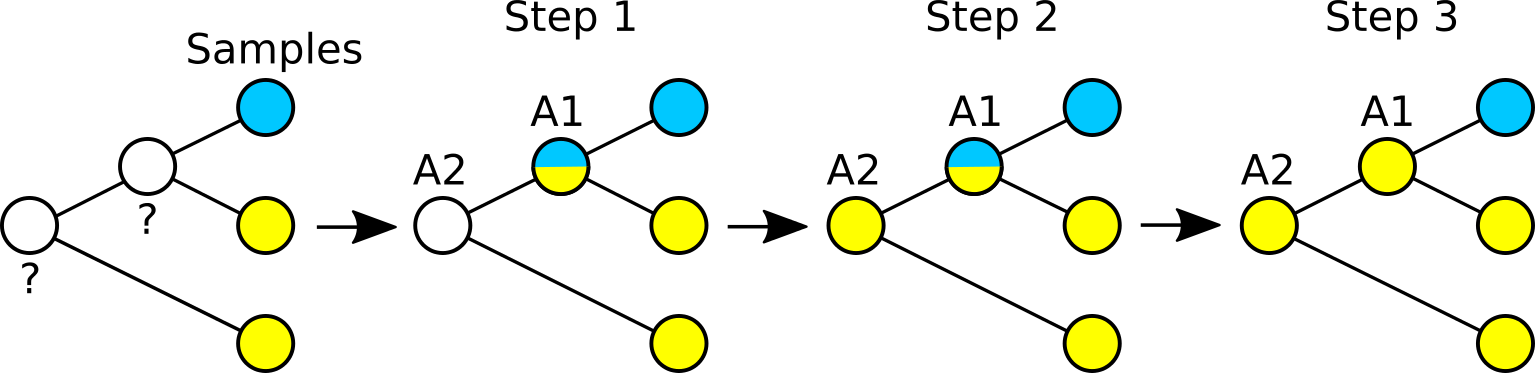
\includegraphics[width=13cm]{img/parsimony.png}
\caption{\label{parsimony} An algorithm that satisfies the
criterion of maximum parsimony. The tree is calculated backwards
until a unique modal value is found. After that the missing
values are recalculated.}
\end{figure}

Figure \ref{parsimony} shows how the most parsimonious solution
is derived for a very simple phylogenetic tree. In this 
example the modal values are calculated backwards in time until
a valid solution is found. After that the tree is recalculated
from the past to the present to find modal values for nodes that
did not have a viable solution before.

In reality the situation is more complicated because in many
cases there simply is no valid solution for a certain marker.
The algorithm that is used by Phyloage works like this:

\begin{enumerate}
\item If possible, modal values that strictly satisfy the
	maximum parsimony criterion are calculated. These are
	the easy cases.
\item The rest of the modal values are calculated by using
	averages and real numbers. This solution should come
	close to the maximum parsimony criterion, at least for
	many samples. In reality this solution is not possible
	because real marker values are restricted to whole numbers.
\item The modal values are mapped to their nearest neighbors
	from the set of real marker values. Still some markers
	can not be calculated because they do not have a unique
	nearest neighbor.
\item All markers that could not be calculated in the top
	node are forced to a real world neighbor value. After
	that the whole tree is recalculated and all markers are
	forced to a real world value.
\end{enumerate}

The algorithm does not necessarily find the best solution
possible, but it should find a good one. For more information
please consult the program's source code documentation
\cite{PhyloageSourceDoc} directly.


\subsection{Phylofriend method}

Phyloage also provides an alternative method to calculate
the modal haplotypes. It is very simple and uses the same
algorithm as the Phylofriend \cite{Phylofriend} program.

\begin{figure}[ht]
\centering
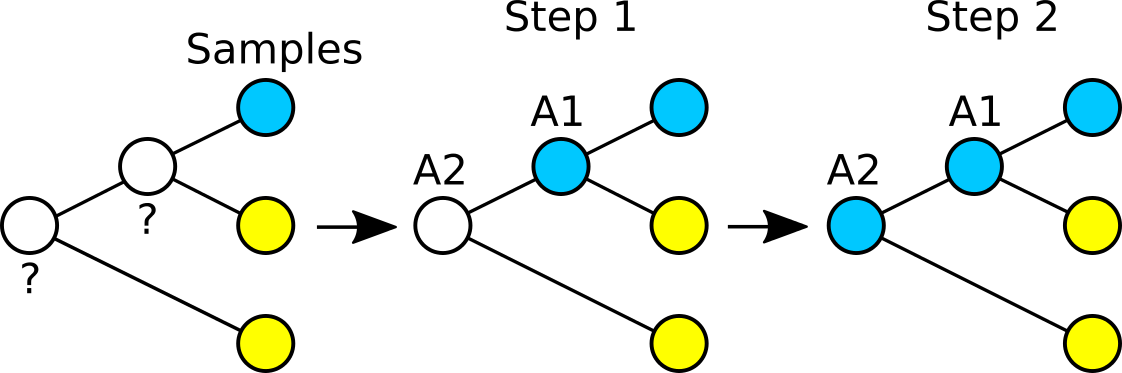
\includegraphics[width=9.5cm]{img/phylofriend.png}
\caption{\label{phylofriend} The Phylofriend method to
determine a modal haplotype is very simple. If a modal
value can't be calculated, it just guesses and continues
the calculation.}
\end{figure}

Figure \ref{phylofriend} illustrates how Phylofriend calculates
a modal haplotype. Generally it chooses the most common value
as the ancestral value. If there is no most common value it
just guesses among the valid ones. This works very well if
a modal haplotype has many samples (at least three) downstream
of it's own. For just two samples the resulting modal haplotype
will be somewhere in between the two sample haplotypes.

This algorithm does not satisfy the maximum parsimony criterion,
but for sparse trees it works better than some might expect.
The reason is that a modal haplotype, that is calculated only
from samples, can not be influenced by older modal values afterwards,
thus eliminating the effect of distant single lineages.

What method to use depends highly on tree structure and
research goals. I am afraid that I can not give a general
recommendation. For sparsely populated trees both methods won't
work very well due to the difficulties involved.
For densely populated trees both methods, maximum parsimony
and Phylofriend, should yield similar results.


\subsection{\label{section_weights}Calculating weights for trees}

Each node of a tree connects several branches and each branch
yields it's own result when calculating the time to the common
ancestor. To calculate the age of a node, the ages of all substream
branches must be taken into account (see figure \ref{weights}).
The first versions of this
program used the average value of all branches. This is simple
but not correct because in this model a single lineage counts as
much as a densely populated branch.

\begin{figure}[ht]
\centering
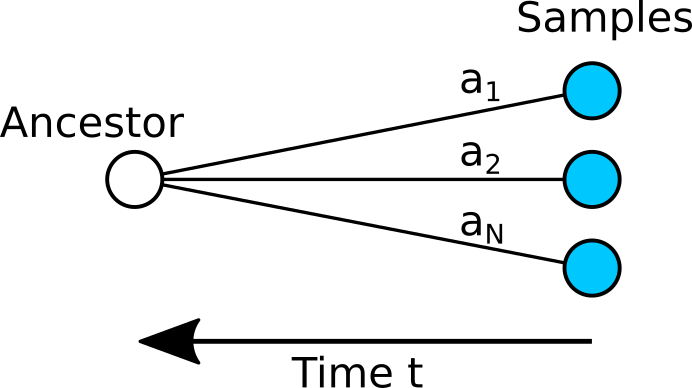
\includegraphics[width=5.9cm]{img/weights.png}
\caption{\label{weights} A number N of samples with different age
estimates $a_1$ to $a_N$ to the common ancestor.}
\end{figure}

To get a better time estimate we must put weights to individual
branches so that single lineages count less and many lineages
count more. To calculate the weights we start with a weighted
time estimate:

\begin{equation}
a = \sum_{i = 1}^{N} w_i a_i    \label{timeestimate}
\end{equation}

\begin{tabular}{ll}
$a$: &  Average time estimate in arbitrary units\\
$a_i$: &  Age estimate of a single branch\\
$w_i$: &  Weight of a branch\\
N: &  Number of substream branches
\end{tabular}
\vspace{1em}

And because we are using a weighted average the sum of all
weights must be equal to 1:

\begin{equation}
\sum_{i = 1}^{N} w_i = 1  \label{normalization}
\end{equation}

How should the weights be calculated? A sensible condition
is that the relative error of our time estimate should be as small as
possible. According to the Gaussian error propagation law
the square of the standard deviation of $a$ is

\begin{equation}
\sigma_a^2 = \sum_{i = 1}^{N} \left(\frac{\partial a}{\partial a_i}
\right)^2 \sigma_i^2  \label{gauss}
\end{equation}

\begin{tabular}{ll}
$\sigma_a^2$: &  Standard deviation of the age estimate a\\
$a_i$: &  Age estimate of branch i\\
$\sigma_i$: &  Standard deviation of $a_i$\\
N: &  Number of substream branches
\end{tabular}
\vspace{1em}

Using equation \ref{timeestimate} we see that the derivatives
are the weights we are looking for:

\begin{equation}
\frac{\partial a}{\partial a_i} = w_i
\end{equation}

And thus we can write equation \ref{gauss} as

\begin{equation}
\sigma_a^2 = \sum_{i = 1}^{N} w_i^2 \sigma_i^2 \label{sigma_square}
\end{equation}

Our goal is to minimize the relative error. So $\sigma_a^2/a$
should be as small as possible. If $\sigma_a^2/a$ is constant
then all it's derivatives become zero and we have a minimum.

Equations \ref{timeestimate} and \ref{sigma_square} look very
similar and indeed if $\sigma_a^2/a$ should be constant we may
write

\begin{eqnarray}
\sigma_a^2 & = & c\ a \\
\Leftrightarrow\ \sum_{i = 1}^{N} w_i^2 \sigma_i^2 & = & c \sum_{i = 1}^{N} w_i a_i
\end{eqnarray}

\begin{tabular}{ll}
a: &  Age\\
$\sigma$: &  Standard deviation\\
w: & Weight\\
c: & Constant (yet unknown)\\
N: & Number of substream branches
\end{tabular}
\vspace{1em}

For symmetry reasons we can concentrate on a single term:

\begin{eqnarray}
w_i^2 \sigma_i^2 & = & c\ w_i a_i\\
\Leftrightarrow\ w_i & = & c\ \frac{a_i}{\sigma_i^2}
\end{eqnarray}

To calculate the constant $c$ we remember that the sum of all
weights must be one (equation \ref{normalization}) and we get 

\begin{equation}
w_i = \frac{1}{\sum_{j=1}^{N}\frac{a_j}{\sigma_j^2}} \ \frac{a_i}{\sigma_i^2}
\end{equation}

This is the formula for the weights. For real-world trees we also
need to calculate the standard deviations of all branches.
This is done in the next section.


\subsection{Calculating standard deviations}


\subsubsection*{Node with samples}

\begin{figure}[ht]
\centering
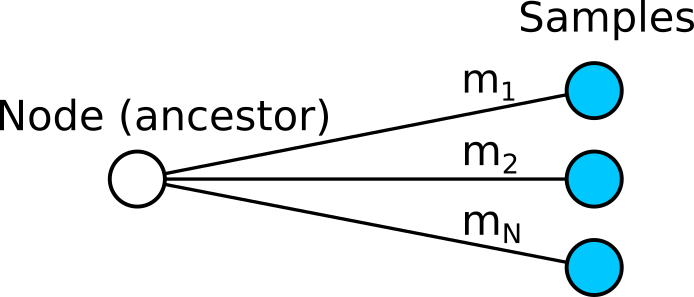
\includegraphics[width=5.9cm]{img/node_with_samples.png}
\caption{\label{node_with_samples} A number N of samples with different
numbers of mutations $m_1$ to $m_N$ to the common ancestral node.}
\end{figure}

It is common that a node is connected to several samples.
The distance from the node to each sample is a number of
mutations $m_i$. Figure \ref{node_with_samples} illustrates
the situation. In this case we can take advantage of the laws
of Gaussian statistics and the standard deviation for the
average number of mutation becomes:

\begin{eqnarray}
\sigma_{\bar{m}} & = & \sqrt{\frac{\bar{m}}{N}}\\
                 & = & \sqrt{\frac{1}{N^2} \sum_{i=1}^{N}m_i}\\
\Leftrightarrow\ \sigma_{\bar{m}}^2 & = & \frac{1}{N^2} \sum_{i=1}^{N}m_i
\end{eqnarray}

\begin{tabular}{ll}
$\sigma_{\bar{m}}$: &  Standard deviation of the average number of mutations\\
$\bar{m}$: & Average number of mutations to the common ancestor\\
$m_i$: &  Number of mutations in branch i\\
N: &  Number of branches
\end{tabular}
\vspace{1em}

This is also true for Poisson statistics but for Poisson
statistics the standard deviation becomes asymmetric to
the average number of mutations.


\subsubsection*{Node with branches}

\begin{figure}[ht]
\centering
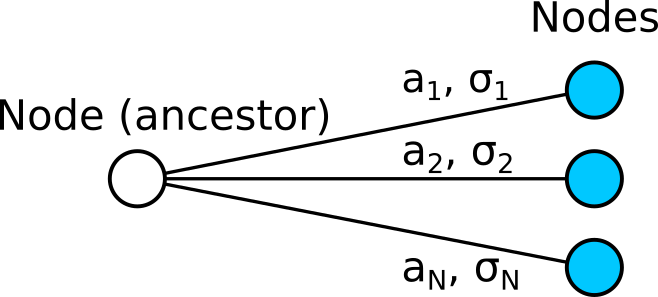
\includegraphics[width=5.9cm]{img/node_with_branches.png}
\caption{\label{node_with_branches} A number N of branches
connected to a node. Each branch has it's own time estimate
$a_i$ and standard deviation $\sigma_i$.}
\end{figure}

A similar but not identical case is when a node is connected
to other nodes by several branches. For each branch a time
estimate and a standard deviation exists and we do not necessarily
know how they were determined (see figure \ref{node_with_branches}).

This is exactly the same situation as in section \ref{section_weights}
and we can write the age estimate as a weighted average:

\begin{equation}
a = \sum_{i = 1}^{N} w_i a_i
\end{equation}

\begin{tabular}{ll}
a: &  Total age estimate in arbitrary units\\
$a_i$: &  Age estimate of a single branch\\
w: &  Weight of a branch\\
N: &  Number of substream branches\\
$\sigma$: & Standard deviation
\end{tabular}
\vspace{1em}

Because we have already calculated this case we can use
equation \ref{sigma_square} to calculate the standard
deviation.

\begin{equation}
\sigma_a^2 = \sum_{i = 1}^{N} w_i^2 \sigma_i^2 
\end{equation}


\subsubsection*{Nodes in a row}

The last case is when three nodes are connected by
two branches in line (see figure \ref{nodes_in_row}).
Again each branch has it's own time estimate and
standard deviation. 

\begin{figure}[ht]
\centering
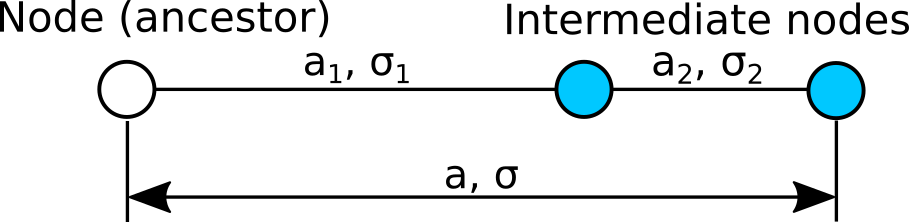
\includegraphics[width=7.7cm]{img/nodes_in_row.png}
\caption{\label{nodes_in_row} Two branches in a row.
Each branch has it's own time estimate
$a_i$ and standard deviation $\sigma_i$.}
\end{figure}

We get the total age estimate $a$ if we add the age estimates
of the two branches together:

\begin{equation}
a = a_1 + a_2
\end{equation}

The standard deviation is determined by the Gaussian error
propagation law:

\begin{eqnarray}
\sigma_a^2 & = & \left( \frac{\partial a}{\partial a_1} \right)^2 \sigma_{a_1}^2
+ \left( \frac{\partial a}{\partial a_2} \right)^2 \sigma_{a_2}^2\\
\Rightarrow\ \sigma_a^2 & = & \sigma_{a_1}^2 + \sigma_{a_2}^2
\end{eqnarray}

\begin{tabular}{ll}
$a_i$: &  Age estimate of a single branch in arbitrary units\\
$a$: & Total age\\
$\sigma$: &  Standard deviation
\end{tabular}
\vspace{1em}











\raggedright
\begin{thebibliography}{bla}

\bibitem{YFullMutationRate} Dmitry Adamov, Vladimir Guryanov,
Sergey Karzhavin, Vladimir Tagankin, Vadim Urasin.
\emph{\href{http://rjgg.molgen.org/index.php/RJGGRE/article/view/151}
{Defining a New Rate Constant for Y-Chromosome SNPs based on Full Sequencing Data}}.
The Russian Journal of Genetic Genealogy
(\foreignlanguage{russian}{Русская версия}),
Vol 6, No 2 (2014)/Vol 7, No 1 (2015).

\bibitem{Fels78} Joseph Felsenstein,
\emph{\href{http://sysbio.oxfordjournals.org/content/27/4/401}
{Cases in which Parsimony or Compatibility Methods will be Positively Misleading}},
Systematic Zoology 27 (4): 401--410, 1978,
\href{http://dx.doi.org/10.1093/sysbio/27.4.401}{doi: 10.1093/sysbio/27.4.401}.

\bibitem{Ham15} David Hamilton,
\emph{\href{http://biorxiv.org/content/early/2015/06/19/020933}
{An accurate genetic clock}},
bioRxiv preprint, first posted online June 15, 2015,
\href{http://dx.doi.org/10.1101/020933}{doi: 10.1101/020933}.

\bibitem{ISOGGTreeR} ISOGG,
\emph{\href{http://www.isogg.org/tree/ISOGG_HapgrpR.html}
{Y-DNA Haplogroup R and its Subclades}}.
Date visited: 2015-10-05.

\bibitem{Kly09} Anatole A. Klyosov,
\emph{\href{http://www.jogg.info/52/files/Klyosov1.pdf}
{DNA Genealogy, Mutation Rates, and Some Historical
Evidence Written in Y-Chromosome, Part I:  Basic Principles and
the Method}}.
Journal of Genetic Genealogy, 5(2):186-216, 2009.

\bibitem{ht35Tree} Sergey Malyshev,
\emph{\href{https://www.familytreedna.com/groups/ht-3-5new/about/results}
{R1b-M269 (P312- U106-) DNA Project (aka ht35 Project) Phylogenetic Tree}}.
R1b-M269 (P312- U106-) DNA Project, Date visited: 2015-10-05.

\bibitem{PhyloageSourceDoc} Dirk Struve,
\emph{\href{https://godoc.org/github.com/yogischogi/phyloage/phylotree}
{Phyloage source code documentation}}, GoDoc, 2016.

\bibitem{Phylofriend} Dirk Struve,
\emph{\href{https://github.com/yogischogi/phylofriend/}{Phylofriend,
a program to calculate genetic distances}}.
Google Project Hosting, 2014; GitHub, 2015.

\bibitem{PhylofriendUserGuide} Dirk Struve,
\emph{\href{https://github.com/yogischogi/phylofriend/blob/master/doc/phylofriend.pdf?raw=true}
{Phylofriend User Guide}}.
Google Project Hosting, 2014; GitHub, 2015.

\bibitem{Wiki-Maximum_parsimony} Wikipedia,
\emph{\href{https://en.wikipedia.org/wiki/Maximum_parsimony_\%28phylogenetics\%29}
{Maximum parsimony}}.
Date accessed: 2016-03-28.

\bibitem{YFullTree} YFull,
\emph{\href{http://yfull.com/tree/}{YFull Phylogenetic Tree}}.
Date visited: 2016-03-01.

\end{thebibliography}

\bibliography{references}
\addcontentsline{toc}{section}{References}
\end{document}
